\section{Introduction and Literature Review}
\label{sec:introduction}

% Question: What is the central problem of this project, in miniature?
% Answer: A transmission spectrum is inferred through a chain of processing
% steps, a real planet provides no known spectrum to score it against, and
% the chain fixes the background early and compresses pixels to one
% dimension, so this project builds a truth-known injector and a joint
% detector-level inference method that makes neither choice.
% Evidence: The argument developed across this introduction.
In conventional analyses, the transmission spectrum of an exoplanet is
inferred from a detector time series through a chain of processing steps:
the detector is calibrated and the background is treated, a spectrum is
extracted from each image, light curves are built from these spectra, and a
transit model is fitted to each light curve. Independent analyses of the
same observation can produce different spectra
\citep{ConstantinouEtAl2023,KirkEtAl2024}, whilst close agreement has also
been reported \citep{LouieEtAl2025}, but neither outcome establishes
absolute accuracy, because for a real planet there is no independently known
spectrum against which the recovered one can be scored. The chain also makes
two structural choices early on. Firstly, the background is estimated before
or during extraction, separately from the transit signal. Secondly, each
detector image is compressed into a one-dimensional spectrum, which can
discard information that the later stages cannot recover. Whether either
choice biases the recovered spectrum can only be answered with data for
which the true spectrum is known. In this project I therefore develop two
connected tools. The first is a detector-level injector, which writes a known
transmission spectrum into the raw data of a real JWST/NIRISS SOSS
observation. The second is NOVA, a forward model which propagates the stellar
spectrum and the transit through a model of the instrument response and fits
them, with the background which remains after detector processing, directly
to the detector pixels, without extracting one-dimensional spectra.

\subsection{Exoplanet atmospheres and transmission spectroscopy}
\label{sec:atmospheres-transmission}
\label{sec:exoplanets-targets}
\label{sec:observing-atmospheres}

% Question: Why study exoplanet atmospheres, and how does transmission
% spectroscopy probe them?
% Answer: Bulk mass and radius leave composition underconstrained, whilst an
% atmosphere records composition, structure, escape and possibly formation;
% wavelength-dependent opacity changes the apparent radius and hence the
% transit depth.
% Evidence: Winn and Fabrycky (2015), Rogers and Seager (2010), Oberg et al.
% (2011), Vidal-Madjar et al. (2003), Madhusudhan (2019), Seager and
% Sasselov (2000), Brown (2001).
Exoplanets span a wide range of sizes, temperatures and orbits, many with no
counterpart in the Solar System \citep{WinnFabrycky2015}. Their mass and
radius constrain the bulk density, but planets with similar masses and radii
can be made of different mixtures of rock, ice and gas
\citep{RogersSeager2010}, and the atmosphere helps to distinguish them
\citep{Madhusudhan2019}: its chemical inventory may carry information about
formation, although not a unique history \citep{ObergEtAl2011}, its thermal
and cloud structure governs how radiation is transported, and escape traces
atmospheric loss \citep{VidalMadjarEtAl2003}. Its signal can be separated
from the light of the star when a planet transits and part of the starlight
passes through its atmospheric limb, a technique known as transmission
spectroscopy. I start with transmission because the geometry of a transit is
well defined and repeats with every orbit, which makes it a convenient setting
in which to test how detector modelling and data reduction affect the
recovered spectrum.
Ignoring for the moment limb darkening, i.e.\ the dimming of the stellar disc
towards its edge, the depth of a transit is approximately
\begin{equation}
  \delta(\lambda) \simeq
  \left[\frac{R_{\mathrm p}(\lambda)}{R_\star}\right]^2 ,
  \label{eq:transit-depth}
\end{equation}
where $\delta(\lambda)$ is the fractional drop in stellar flux during
transit, $R_{\mathrm p}(\lambda)$ is the effective radius of the planet at
wavelength $\lambda$ and $R_\star$ is the radius of the star. The effective
radius is larger where the atmosphere is more opaque, and so absorption by
atoms, molecules, clouds and aerosols imprints wavelength-dependent structure
on the transit depth \citep{SeagerSasselov2000,Brown2001}, as shown in
Figure~\ref{fig:transmission-spectroscopy}.

\begin{figure*}[t]
  \centering
  \begin{tikzpicture}[x=1cm,y=1cm,font=\footnotesize]
  \path[use as bounding box] (0,0) rectangle (17.2,5.15);

  % Panel frames and titles
  \draw[black!25,line width=0.4pt] (0.05,0.10) rectangle (8.25,5.00);
  \draw[black!25,line width=0.4pt] (8.70,0.10) rectangle (17.15,5.00);
  \node[anchor=west,font=\bfseries] at (0.25,4.72)
    {(a) Transit geometry};
  \node[anchor=west,font=\bfseries] at (8.90,4.72)
    {(b) Wavelength-dependent transit depth};

  % Star
  \shade[inner color=yellow!15,outer color=transitstar]
    (1.60,2.60) circle (1.23);
  \draw[transitstar!70!black,line width=0.5pt]
    (1.60,2.60) circle (1.23);
  \node[anchor=north] at (1.60,1.20) {Host star};

  % Wavelength-labelled stellar rays before and after the atmosphere
  \draw[transitstar!80!black,line width=1.15pt]
    (2.72,3.10) -- (4.10,3.10);
  \draw[transitabsorb,line width=0.55pt,->]
    (5.32,3.10) -- (7.72,3.10);
  \node[anchor=south,text=transitabsorb] at (3.42,3.13)
    {$\lambda_{\rm high}$};

  \draw[transitstar!80!black,line width=1.15pt]
    (2.72,2.02) -- (4.16,2.02);
  \draw[transitatmos,line width=0.95pt,->]
    (5.27,2.02) -- (7.72,2.02);
  \node[anchor=north,text=transitatmos] at (3.43,1.98)
    {$\lambda_{\rm low}$};

  % Opaque planet and wavelength-dependent atmospheric radii
  \fill[transitatmos!12] (4.72,2.60) circle (0.78);
  \draw[transitabsorb,dashed,line width=1.05pt]
    (4.72,2.60) circle (0.78);
  \draw[transitatmos,line width=1.05pt]
    (4.72,2.60) circle (0.61);
  \fill[transitplanet] (4.72,2.60) circle (0.45);
  \draw[black,line width=0.45pt] (4.72,2.60) circle (0.45);

  \draw[transitabsorb,dashed,line width=1.05pt]
    (5.30,4.08) -- (5.86,4.08);
  \node[anchor=west,text=transitabsorb] at (5.96,4.08)
    {larger $R_{\rm p}(\lambda_{\rm high})$};
  \draw[transitatmos,line width=1.05pt]
    (5.30,3.72) -- (5.86,3.72);
  \node[anchor=west,text=transitatmos] at (5.96,3.72)
    {smaller $R_{\rm p}(\lambda_{\rm low})$};

  \draw[black!60,->,line width=0.55pt]
    (5.82,2.59) -- (5.32,2.67);
  \node[anchor=west,align=left] at (5.90,2.58)
    {atmospheric\\annulus};

  \node[anchor=north,align=center] at (4.72,1.58)
    {Planet and\\atmospheric annulus};
  \node[anchor=north,align=center] at (7.35,1.88)
    {toward the\\observer};

  % Spectrum axes
  \draw[->,line width=0.65pt] (9.45,0.83) -- (16.78,0.83);
  \draw[->,line width=0.65pt] (9.45,0.83) -- (9.45,4.38);
  \node[anchor=north] at (13.10,0.66) {Wavelength, $\lambda$};
  \node[rotate=90,anchor=south] at (8.92,2.63)
    {Transit depth, $\delta(\lambda)$};

  % Illustrative transmission spectrum
  \draw[black!15,densely dotted] (9.45,1.43) -- (16.64,1.43);
  \draw[black!20,densely dotted] (9.45,2.75) -- (16.64,2.75);
  \draw[transitplanet,line width=1.35pt]
    plot[smooth,tension=0.72] coordinates {
      (9.52,1.47) (9.88,1.50) (10.22,1.62) (10.56,2.15)
      (10.90,1.70) (11.28,1.52) (11.65,1.58) (12.03,1.86)
      (12.38,3.05) (12.73,1.91) (13.08,1.56) (13.48,1.49)
      (13.88,1.68) (14.27,2.19) (14.65,1.73) (15.03,1.62)
      (15.39,2.00) (15.76,3.48) (16.10,2.03) (16.50,1.57)
    };

  % Link spectral extrema to the two atmospheric radii in panel (a)
  \fill[transitabsorb] (12.38,3.05) circle (0.065);
  \draw[transitabsorb,densely dashed] (12.38,0.84) -- (12.38,3.05);
  \node[anchor=south,text=transitabsorb,align=center]
    at (12.38,3.18) {higher opacity\\deeper transit};

  \fill[transitatmos] (13.48,1.49) circle (0.065);
  \draw[transitatmos,densely dashed] (13.48,0.84) -- (13.48,1.49);
  \node[anchor=west,text=transitatmos,align=left]
    at (13.63,1.44) {lower opacity\\shallower transit};

  \node[anchor=east,align=right,font=\scriptsize] at (16.68,4.20)
    {$\mathrm{opacity}\!\uparrow\;\Rightarrow\;
      R_{\rm p}(\lambda)\!\uparrow\;\Rightarrow\;
      \delta(\lambda)\!\uparrow$};
\end{tikzpicture}

  \caption{Principle of transmission spectroscopy. (a) During transit, the
  opaque body of the planet blocks starlight, whilst a small fraction of the
  starlight passes through its atmospheric annulus. The altitude at which
  the atmosphere becomes opaque, and hence the apparent radius of the
  planet, depends on wavelength. (b) Where the atmosphere is more opaque,
  $R_{\mathrm p}(\lambda)$ is larger and the transit is deeper. The spectrum
  shown is schematic and does not represent a particular planet or
  instrument.}
  \label{fig:transmission-spectroscopy}
\end{figure*}

% Question: Why are transmission signals small, why begin with hot Jupiters,
% and why is the accuracy of the spectrum itself the focus?
% Answer: Only a thin annulus is probed; hot Jupiters give strong signals
% which make reduction errors easier to diagnose; atmospheric
% characterisation is an inverse problem that starts from an inferred
% spectrum.
% Evidence: Seager and Sasselov (2000), Brown (2001), Charbonneau et al.
% (2002), Madhusudhan (2019), Deming et al. (2005), Knutson et al. (2007),
% Coulombe et al. (2023), Mikal-Evans et al. (2023), Kempton et al. (2023),
% Gressier et al. (2024), Splinter et al. (2025), Rackham et al. (2018),
% Barstow and Heng (2020).
Only the starlight which passes through a thin annulus around the planet
probes its atmosphere, and so the signal is a small fraction of the stellar
flux, largest for planets which are large relative to their star and have hot,
hydrogen-rich, low-gravity atmospheres \citep{SeagerSasselov2000,Brown2001}. Hot Jupiters are therefore
especially favourable targets \citep{Brown2001,Madhusudhan2019}, and the
first detection of an exoplanet atmosphere was the sodium absorption of
HD~209458~b \citep{CharbonneauEtAl2002}. Their strong signals also make
errors in data reduction easier to diagnose, and so methods are best
developed on them before being tested, and if necessary revalidated, on
smaller and cooler planets. Transmission is one of three time-series geometries: secondary
eclipses isolate the emission from the dayside
\citep{DemingEtAl2005,CoulombeEtAl2023,GressierEtAl2024}, and phase curves
constrain the day--night contrast, heat redistribution and longitudinal
structure \citep{KnutsonEtAl2007,MikalEvansEtAl2023,KemptonEtAl2023,
SplinterEtAl2025}; both are planned as later applications of this work.
Since different combinations of abundances, temperature, clouds, hazes and
stellar heterogeneity can produce similar spectra
\citep{RackhamEtAl2018,Madhusudhan2019}, atmospheric characterisation is an
inverse problem \citep{BarstowHeng2020}, and it starts from a spectrum which
is itself inferred from the detector data, so that a
retrieval can be statistically precise whilst inheriting a bias from the
spectrum. This work is mainly concerned with this first stage, i.e.\ with
how accurately the spectrum itself is recovered, although its last objective
(Section~\ref{sec:research-question}) also asks how errors in it propagate
into the retrieval.

\subsection{JWST, NIRISS/SOSS, and the WASP-17~b case study}
\label{sec:jwst-soss-wasp17}
\label{sec:arecibo-to-jwst}
\label{sec:soss-wasp17}

% Question: Where did the targets and techniques come from, and what changed
% with JWST?
% Answer: Three decades of discovery produced thousands of planets and bright
% targets; HST and Spitzer established the techniques but stitched broad
% spectra across instruments and epochs; JWST covers several absorbers in
% one mode and visit.
% Evidence: Wolszczan and Frail (1992), Mayor and Queloz (1995), Borucki et
% al. (2010), Ricker et al. (2015), NASA Exoplanet Archive (2026), Deming et
% al. (2005), Charbonneau et al. (2005), Knutson et al. (2007), Sing et al.
% (2016), Gardner et al. (2006), Rigby et al. (2023).
Three decades of discovery, from the pulsar planets
\citep{WolszczanFrail1992} and 51~Pegasi~b \citep{MayorQueloz1995} to the
Kepler and TESS surveys \citep{BoruckiEtAl2010,RickerEtAl2015}, have produced
more than 6,000 confirmed exoplanets \citep{NASAExoplanetArchive2026},
including many around the bright, nearby hosts which are most favourable for follow-up.
HST and Spitzer established the techniques of atmospheric characterisation
\citep{DemingEtAl2005,CharbonneauEtAl2005,KnutsonEtAl2007}, and the
ten-planet survey of \citet{SingEtAl2016} found a continuum from clear to
cloudy atmospheres, but broad wavelength coverage was commonly assembled
from different instruments at different epochs. JWST, a 6.5-metre,
cryogenic, infrared-optimised observatory \citep{GardnerEtAl2006} whose
performance met or exceeded its requirements in most areas
\citep{RigbyEtAl2023}, can measure smaller changes in transit depth and
cover several absorbers within a single mode and visit. This project starts
with its NIRISS Single Object Slitless Spectroscopy (SOSS) mode
\citep{AlbertEtAl2023}, and with a single observation: a complete transit of
WASP-17~b \citep{LouieEtAl2025}.

% Question: What makes SOSS useful and difficult, and how precise is it?
% Answer: Broad coverage at R~650 with defocused, curved, partly overlapping
% orders; 20 ppm white-light scatter in commissioning, but 46--73 ppm median
% per-channel uncertainties across three reductions of WASP-17 b.
% Evidence: Albert et al. (2023), Holmberg and Madhusudhan (2023), Louie et
% al. (2025).
SOSS uses the GR700XD disperser, a grism combined with a cross-dispersing
prism, which spreads the light into several spectral orders covering
approximately $0.6$--$2.8\,\mu\mathrm{m}$ at a resolving power of about
$R=650$ at $1.25\,\mu\mathrm{m}$ \citep{AlbertEtAl2023}. The prism curves the
orders on the detector, and because limited mechanical clearance restricted
the angles of the prism and grism, the first two orders partly overlap, which
makes spectral extraction particularly difficult \citep{AlbertEtAl2023}. A
weak cylindrical lens spreads the light over roughly 23 detector rows, so
that bright stars can be observed without saturating, and the bandpass
contains several water bands, the potassium doublet and regions sensitive to
other absorbers and to clouds and hazes
\citep{AlbertEtAl2023,HolmbergMadhusudhan2023,LouieEtAl2025}. The curved
footprints of the two orders, the traces, are shown in
Figure~\ref{fig:soss-detector-orders}. During commissioning, a detrended SOSS
white-light time series of a standard star reached a scatter of about 20~ppm
when averaged over
40-minute intervals \citep{AlbertEtAl2023}, but a spectral channel contains
fewer photons, and for WASP-17~b three reductions of the same observation
reported median uncertainties of 46--73~ppm per channel across orders 1 and 2
\citep{LouieEtAl2025}, which shows that the precision assigned to a spectrum
depends on the analysis, at a level relevant to the atmospheric signal.

\begin{figure*}[t]
  \centering
  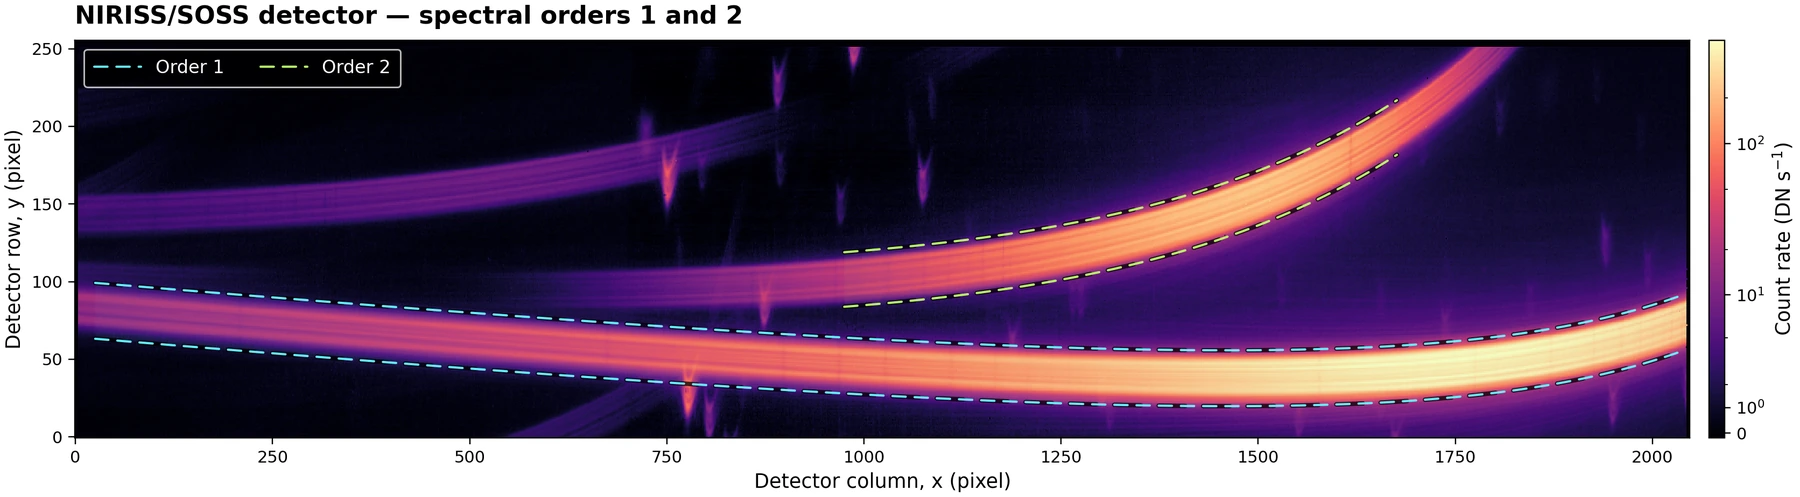
\includegraphics[width=\textwidth]{figures/niriss_soss_detector_orders.png}
  \caption{Median NIRISS/SOSS detector image, showing the curved traces of
  the first- and second-order spectra. The cyan and green dashed lines mark
  the pixel supports which NOVA fits for orders 1 and 2, respectively. An
  inverse hyperbolic sine (\(\operatorname{asinh}\)) stretch keeps both the
  bright cores of the traces and their fainter wings visible; the colour bar
  gives the count rate in \(\mathrm{DN\,s^{-1}}\).}
  \label{fig:soss-detector-orders}
\end{figure*}

% Question: What has SOSS delivered, what difficulties does it expose, and
% why WASP-17 b?
% Answer: Molecular, atomic and cloud signatures, but analyses must treat
% overlapping orders, field stars and a structured background; WASP-17 b
% has earlier constraints, a complete SOSS transit and three reductions.
% Evidence: Feinstein et al. (2023), Albert et al. (2023), Radica et al.
% (2023), Holmberg and Madhusudhan (2023), Anderson et al. (2010), Alderson et
% al. (2022), Louie et al. (2025), Espinoza et al. (2019), Espinoza (2022),
% Radica (2024).
The first SOSS analyses recovered detailed structure, such as the water
bands, potassium and clouds of WASP-39~b \citep{FeinsteinEtAl2023}. Besides
the difficulties which every JWST transit analysis faces, SOSS adds three of
its own: its curved orders overlap, the
spectra of field stars also fall on the detector because the mode is
slitless, and the zodiacal background has a sharp step near detector column
700 \citep{AlbertEtAl2023,RadicaEtAl2023,HolmbergMadhusudhan2023}. WASP-17~b, the first case study, is a hot Jupiter. Its
low density and gravity give it an extended atmosphere
\citep{AndersonEtAl2010}, and a $0.3$--$5\,\mu\mathrm{m}$ spectrum from HST
and Spitzer still allowed both a high- and a low-metallicity interpretation
\citep{AldersonEtAl2022}. \citet{LouieEtAl2025} then analysed a complete SOSS
transit with three reductions: Ahsoka, which they introduced;
\texttt{transitspectroscopy} \citep{Espinoza2022TransitSpectroscopy} with
\texttt{juliet} \citep{EspinozaEtAl2019}; and supreme-SPOON
\citep{RadicaEtAl2023}, now distributed as exoTEDRF \citep{Radica2024}. The
three spectra agreed closely over most of the bandpass and constrained the
water abundance more tightly than the earlier data had, which, together with
the earlier observations, makes WASP-17~b a strong case for a controlled
comparison of methods.

\subsection{From detector integrations to the validation problem}
\label{sec:detector-to-validation}
\label{sec:detector-to-spectrum}
\label{sec:validation-problem}

\begin{figure*}[t]
  \centering
  \begin{tikzpicture}[x=1cm,y=1cm,font=\footnotesize]
  \path[use as bounding box] (0,0) rectangle (17.2,5.25);

  % Panel frames and headings
  \draw[black!22,line width=0.4pt] (0.05,0.12) rectangle (4.95,5.10);
  \draw[black!22,line width=0.4pt] (5.20,0.12) rectangle (17.15,5.10);
  \node[anchor=west,font=\bfseries] at (0.28,4.82)
    {(a) Detector ramp};
  \node[anchor=west,font=\bfseries] at (5.44,4.82)
    {(b) Extraction-first reduction};

  % Ramp sampling within an integration
  \draw[->,line width=0.65pt] (0.82,0.92) -- (4.38,0.92);
  \draw[->,line width=0.65pt] (0.82,0.92) -- (0.82,4.22);
  \node[anchor=north] at (2.60,0.78) {Time within integration};
  \node[rotate=90,anchor=center] at (0.30,2.55)
    {Accumulated counts};

  \draw[transitatmos!75!black,line width=1.0pt]
    (1.03,1.20) -- (3.83,3.79);
  \foreach \x/\y/\lab in {
    1.18/1.32/G1,
    1.72/1.82/G2,
    2.26/2.32/G3,
    2.80/2.82/G4,
    3.34/3.32/G5}
  {
    \fill[transitatmos] (\x,\y) circle (0.075);
    \node[anchor=south,font=\scriptsize,text=transitatmos!70!black]
      at (\x,\y+0.10) {\lab};
  }
  \draw[->,transitabsorb,line width=0.75pt]
    (3.58,2.66) -- (3.08,3.08);
  \node[anchor=west,text=transitabsorb,align=left,font=\scriptsize]
    at (3.56,2.40) {slope =\\count rate};
  % Reusable box dimensions and top workflow row
  \draw[rounded corners=2pt,fill=transitatmos!8,draw=transitatmos!65,
    line width=0.55pt] (5.44,3.18) rectangle (7.76,4.23);
  \node[align=center,font=\scriptsize] at (6.60,3.705)
    {Count-rate images\\at $t_1,t_2,\ldots$};

  \draw[rounded corners=2pt,fill=transitatmos!8,draw=transitatmos!65,
    line width=0.55pt] (8.05,3.18) rectangle (10.80,4.23);
  \node[align=center,font=\scriptsize] at (9.425,3.705)
    {Detector corrections\\background and $1/f$\\trace and bad pixels};

  \draw[rounded corners=2pt,fill=transitstar!10,draw=transitstar!75!black,
    line width=0.55pt] (11.09,3.18) rectangle (13.84,4.23);
  \node[align=center,font=\scriptsize] at (12.465,3.705)
    {Spectral extraction\\box, optimal, or\\forward model};

  \draw[rounded corners=2pt,fill=transitstar!10,draw=transitstar!75!black,
    line width=0.55pt] (14.13,3.18) rectangle (16.91,4.23);
  \node[align=center,font=\scriptsize] at (15.52,3.705)
    {One-dimensional spectra\\for each integration};

  \draw[->,line width=0.65pt] (7.76,3.705) -- (8.05,3.705);
  \draw[->,line width=0.65pt] (10.80,3.705) -- (11.09,3.705);
  \draw[->,line width=0.65pt] (13.84,3.705) -- (14.13,3.705);
  \node[anchor=north,font=\scriptsize,text=transitabsorb]
    at (12.465,3.10) {spectral compression};

  % Continue the workflow on a second row from right to left
  \draw[rounded corners=2pt,fill=black!3,draw=black!38,line width=0.55pt]
    (14.13,1.38) rectangle (16.91,2.43);
  \node[align=center] at (15.52,1.905)
    {Wavelength\\binning};

  \draw[rounded corners=2pt,fill=black!3,draw=black!38,line width=0.55pt]
    (11.09,1.38) rectangle (13.84,2.43);
  \node[align=center] at (12.465,1.905)
    {Spectral\\light curves};

  \draw[rounded corners=2pt,fill=transitabsorb!9,draw=transitabsorb!70,
    line width=0.55pt] (8.05,1.38) rectangle (10.80,2.43);
  \node[align=center,font=\scriptsize] at (9.425,1.905)
    {Transit inference\\pipeline-specific\\nuisance model};

  \draw[rounded corners=2pt,fill=transitplanet!5,draw=transitplanet!65,
    line width=0.55pt] (5.44,1.38) rectangle (7.76,2.43);
  \node[align=center] at (6.60,1.905)
    {Transmission\\spectrum};

  \draw[->,line width=0.65pt]
    (16.91,3.705) -- (17.01,3.705) -- (17.01,2.64) --
    (15.52,2.64) -- (15.52,2.43);
  \draw[->,line width=0.65pt] (14.13,1.905) -- (13.84,1.905);
  \draw[->,line width=0.65pt] (11.09,1.905) -- (10.80,1.905);
  \draw[->,line width=0.65pt] (8.05,1.905) -- (7.76,1.905);

  \node[anchor=north,align=center,font=\scriptsize,text=black!65]
    at (11.30,1.05)
    {Detector pixels are no longer available to the downstream light-curve fit};
\end{tikzpicture}

  \caption{Conceptual structure shared by extraction-first JWST/NIRISS SOSS
  reductions. (a) Within an integration, the detector is read
  nondestructively several times, and each read (group) samples the
  accumulated charge. A cosmic ray adds a step, which the several groups make
  visible, so the count rate can be fitted from the unaffected differences
  between reads. (b) After the background and noise have been treated,
  extraction compresses each count-rate image into a one-dimensional
  spectrum; binning in wavelength gives one light curve per channel, and a
  transit fit to each gives the depths which make up the transmission
  spectrum. The implementation and order of these steps, including whether
  an operation is applied to groups or to count rates, differ between
  pipelines.}
  \label{fig:extraction-first-workflow}
\end{figure*}

% Question: What is the shared extraction-first chain, and where do
% pipelines differ?
% Answer: Detector corrections and ramp fitting, background and noise
% treatment, extraction, per-channel light curves and transit fitting;
% implementations differ at almost every step, including the systematics
% models of the three WASP-17 b branches.
% Evidence: Albert et al. (2023), Bell et al. (2022), Radica et al. (2023),
% Holmberg and Madhusudhan (2023), Louie et al. (2025).
To see where the structural choices enter, it helps to follow the data from
the detector. During each integration, the detector is read nondestructively
several times, each read here being recorded as one group, and a fit to the
accumulating charge gives a count rate for each pixel, so that a visit
produces a time series of two-dimensional count-rate images
\citep{AlbertEtAl2023}. The conventional analyses then follow the
extraction-first workflow of Figure~\ref{fig:extraction-first-workflow}. The raw reads are calibrated with the JWST pipeline or a variant of it, which
flags saturated data, subtracts the bias, applies the reference-pixel,
nonlinearity and dark-current corrections, detects jumps such as cosmic
rays and fits each ramp, with the low-frequency ($1/f$) readout noise
corrected either before ramp fitting or on the count-rate images. Later steps
treat the flat field, background, field stars and bad pixels, an extraction
converts each image into a one-dimensional spectrum
\citep{Horne1986,DarveauBernierEtAl2022}, and a transit model is fitted to the
light curve of each wavelength channel
\citep{BellEtAl2022,RadicaEtAl2023,LouieEtAl2025}. Implementations differ in
the order of these operations and in the choices at each step, for example
in the jump threshold, where the $1/f$ correction is applied, how the
background is scaled and field stars are treated, and in the trace profiles,
extraction widths, limb-darkening priors and systematics models
\citep{RadicaEtAl2023,HolmbergMadhusudhan2023,LouieEtAl2025}. For WASP-17~b,
for instance, the remaining time dependence was modelled with polynomial
trends and a multiplicative noise term by Ahsoka, which uses the Eureka!
framework \citep{BellEtAl2022}, with a Mat\'ern-$3/2$ Gaussian process by
\texttt{transitspectroscopy}, whilst supreme-SPOON fitted no systematics function, only an
additive uncertainty term \citep{LouieEtAl2025}.

% Question: What can a comparison of reductions establish?
% Answer: Disagreement shows sensitivity and agreement shows
% reproducibility, but neither identifies the more accurate spectrum, and a
% good pixel fit does not prove a correct decomposition.
% Evidence: Constantinou et al. (2023), Kirk et al. (2024), Louie et al.
% (2025), Bell et al. (2022), Radica et al. (2023), Darveau-Bernier et al.
% (2022).
What, then, can a comparison of the resulting spectra establish? When
reductions disagree, the spectrum is shown to be sensitive to the analysis:
for the 3--5~$\mu\mathrm{m}$ NIRSpec spectrum of WASP-39~b, differences
between reductions changed the retrieved abundances by up to about an order
of magnitude \citep{ConstantinouEtAl2023}, and for the sub-Earth GJ~341~b,
three reductions all detected no atmosphere, yet two produced weak candidate
features at different wavelengths, and so favoured different molecules
\citep{KirkEtAl2024}. A difference does not, however, identify which spectrum
is more accurate. When reductions agree, as the three WASP-17~b reductions do,
this is strong evidence of reproducibility, and where they made different
choices it suggests that the net effect of those choices was small relative
to the quoted uncertainties, although individual effects could cancel. They do, however, start from the same
observation, use the same reference files and in part share software
\citep{BellEtAl2022,RadicaEtAl2023,LouieEtAl2025}, and so agreement cannot
reveal an assumption which all of them share. Both cases come back to the
same problem: a real planet has no independently known spectrum, and so
neither measures the absolute error of a recovery. Nor do the residuals of a
fit, because an incorrect split of the observed light into source, background
and instrument terms can still fit the pixels well. Absolute validation
therefore requires data for which the generating spectrum is known.
Simulated SOSS observations have been used to validate individual steps;
ATOCA, for example, recovers the input spectrum to within 10~ppm when its
calibration inputs are correct \citep{DarveauBernierEtAl2022}. Such
simulations, however, only contain the noise and background that were
modelled.

\FloatBarrier
\subsection{Two structural hypotheses and the response of this project}
\label{sec:structural-limitations-inference}
\label{sec:structural-limitations}
\label{sec:benchmark-and-nova}

% Question: How do published methods treat the background, and when is
% joint inference identifiable?
% Answer: They subtract it before extraction or refine it during extraction,
% but none infers it jointly with the transit; source and background are
% degenerate in one pixel but separable across many pixels sharing one depth.
% Evidence: Louie et al. (2025), Holmberg and Madhusudhan (2023).
Whilst the lack of a ground truth affects every method, the two structural
choices introduced at the start of this section are specific to the
conventional chain, and I treat each as a hypothesis about where recovery
error could enter, without presuming that either causes a bias. The first is
that treating the background separately from the transit could bias the
recovered spectrum. In the Ahsoka and supreme-SPOON reductions of WASP-17~b,
a scaled STScI model of the zodiacal background was subtracted before the
light curves were fitted, with its scaling fixed in the transit fit, and the
\texttt{transitspectroscopy} reduction followed the same order
\citep{LouieEtAl2025}. JExoRES is an important
exception, since it fits a residual background level together with the fluxes
of the overlapping orders \citep{HolmbergMadhusudhan2023}, but even there the
background is fitted during the extraction of a stellar spectrum, and the
transit only in the next stage. The important question is therefore whether
the background and the wavelength-dependent transit are inferred together.
Because the transit dims the starlight but not the additive background, the
difference between in-transit and out-of-transit images shows where the
starlight falls. In a single pixel, however, the fractional depth and a
constant additive term cannot be separated, since the data only fix the
out-of-transit level and the absolute size of the dip. The split becomes
possible because the same depth applies to many pixels whose ratios of
starlight to background differ, provided that the background is described by
far fewer parameters than there are pixels and does not itself vary in time
like a transit. This information is lost once the pixels are summed into a
light curve, and none of the published implementations considered here infers
the background jointly with the transit in one likelihood over the detector
pixels \citep{HolmbergMadhusudhan2023,LouieEtAl2025}.

% Question: How can a background error bias the spectrum?
% Answer: The background adds whilst the transit multiplies, so misallocated
% flux changes the fractional depth; the downstream fit cannot correct it
% without a propagated covariance.
% Evidence: Louie et al. (2025), Kelson (2003), Radica et al. (2023),
% Holmberg and Madhusudhan (2023).
After extraction, all that remains of the background is any residual error
and its propagated uncertainty. The three WASP-17~b branches report
per-channel uncertainties and downstream noise terms, but do not describe
passing on a wavelength-correlated covariance of the background subtraction,
and so the transit fit cannot correct an error in how the counts were divided
between the star and the background. Such an error matters because the
background is added to the starlight, whereas the transit multiplies it: if
a constant amount of flux is wrongly assigned to the background, the
out-of-transit stellar flux is wrong by the same amount, and the depth,
measured as a fraction of this flux, is biased; too much flux in the
background, for example, makes the transit appear deeper. An error which
varies across the detector can change spectral offsets, slopes or local
features. Classical two-dimensional spectroscopy has shown the value of
modelling the background in the native detector geometry \citep{Kelson2003},
and for SOSS the problem also includes structured zodiacal light, field-star
spectra, masked pixels and $1/f$ noise
\citep{RadicaEtAl2023,HolmbergMadhusudhan2023}.

% Question: When does compression to one dimension lose information, and
% what remains after ATOCA?
% Answer: A compressed product preserves the pixel likelihood only if its
% model is right and a suitable covariance is carried forward; ATOCA models
% the order overlap but still estimates the spectrum before the transit.
% Evidence: Horne (1986), Bolton and Schlegel (2010), Bolton et al. (2012),
% Darveau-Bernier et al. (2022), Radica et al. (2022), Bell et al. (2022),
% Radica et al. (2023).
The second hypothesis concerns the compression of detector pixels into
one-dimensional spectra. Extraction need not lose information: if the
spatial profile, background, response, bad-pixel mask and noise model are
all correct, the optimal extraction of \citet{Horne1986}, which weights the
pixels of each column by the profile divided by the variance, is an efficient
summary, and \citet{BoltonSchlegel2010} showed that a one-dimensional product
preserves the pixel-level likelihood if it is delivered with a suitable
covariance and resolution description \citep{BoltonEtAl2012}. Conversely, if
the trace, the blending of neighbouring wavelengths, the background, the
bad-pixel treatment or the decomposition into orders is fixed incorrectly,
and this covariance is not carried forward, a later light-curve fit cannot
recover what was lost. For SOSS this is hardest where the two orders overlap.
The ATOCA algorithm models every pixel as the sum of both orders, produced by
one incident spectrum; for a typical box extraction, ignoring the
contamination between the orders would bias transit spectra by about 1\% of
the strength of their features \citep{DarveauBernierEtAl2022}. Its accuracy
depends on its calibration inputs, of which the APPLESOSS package
\citep{RadicaEtAl2022} estimates the spatial profiles from the observation
itself. Even so, ATOCA keeps
the two-stage structure, since the transit is only fitted after the spectrum
of each integration has been estimated
\citep{DarveauBernierEtAl2022,BellEtAl2022,RadicaEtAl2023}. This ordering is
practical, and it may be entirely adequate, but the transit model cannot then
help, within one likelihood, to separate the starlight, the background and
the overlapping orders. Whether this causes a meaningful bias in SOSS spectra
is an empirical question, which the benchmark below is designed to answer.

% Question: How can absolute recovery accuracy be measured, and how does
% NOVA respond to the two hypotheses?
% Answer: A truth-known injection into real raw data, identical inputs, and
% truth revealed after each prediction is fixed; NOVA fits one shared
% spectrum, continuum and background in detector space, but depends on three
% earlier steps.
% Evidence: The benchmark design and NOVA forward model in the Methods.
The validation problem and these two hypotheses together motivate a
benchmark at the detector level. An injector writes a known transmission
spectrum into the raw data of the integrations taken before the real transit
of WASP-17~b, so that the background, noise, detector flags and field sources
are real whilst the injected spectrum is known. The injected transit dims
only the light which the injector assigns to the target star, and since it is
not known how much of the faint light far from the traces belongs to the
star, I bracket this between a lower and an upper estimate
(Section~\ref{sec:injector}). Every method is given the same injected raw
frames and the same geometry priors, and the injected spectrum is only
revealed once each method has fixed its prediction, so that the recovery
error can be measured directly. NOVA is the recovery method developed alongside this benchmark.
It evaluates a forward model in detector space, in which one transmission
spectrum, shared by orders 1 and 2, is propagated through the instrument
response and fitted together with the limb darkening, the stellar continuum
and the additive background, and only the starlight is multiplied by the
transit. This keeps the physical distinction between source and background,
and lets many pixels, in both orders, constrain the same spectrum. NOVA is
not free of earlier steps, however (Section~\ref{sec:nova}). Firstly, the
detector processing subtracts a scaled background model before the fit,
although the background which remains is fitted again together with the
transit. Secondly, the spatial response is estimated from the same data.
Finally, the transit geometry comes from a white-light fit to optimally
extracted light curves. A good fit to the pixels does not prove that star,
background and transit were separated correctly, and so NOVA cannot validate
itself; the benchmark supplies the missing truth, and can show whether the
established pipelines already recover the injected spectra without a
detectable bias and whether NOVA improves on them. Where every method fails,
it points instead to an inadequate instrument model or injector.

\subsection{Research question and objectives}
\label{sec:research-question}

% Question: What is the central research question?
% Answer: Kept verbatim from the agreed version.
% Evidence: The validation problem and structural hypotheses above.
The central research question of this project is:
\begin{quote}
\raggedright\itshape
How accurately and robustly can JWST/NIRISS SOSS transmission spectra
be recovered from detector-level time-series observations, and can joint
detector-level inference reduce biases associated with background treatment and
extraction-first analysis?
\end{quote}

To make this question testable, I divide it into four objectives:
\begin{enumerate}[label=\arabic*.,leftmargin=1.5em]
  \item develop an independent detector-level benchmark with known injected
  transmission spectra;
  \item develop NOVA as a joint detector-level inference method for
  NIRISS/SOSS transmission spectroscopy;
  \item compare NOVA with extraction-based analyses under controlled
  observing conditions and atmospheric scenarios; and
  \item identify the detector, calibration and modelling assumptions which
  limit recovery accuracy, and determine how these limitations propagate into
  atmospheric interpretation.
\end{enumerate}

% Question: What is the scope of the present assessment?
% Answer: It defines the problem, documents the methods and plans the
% experiments, reporting only results whose checks are complete.
% Evidence: The Methods, Results and Research Plan sections.
WASP-17~b is only the first case study: the production stage of the
benchmark (Section~\ref{sec:envelope}) will repeat the injections in five further
SOSS visits, of HAT-P-26, WASP-39, HAT-P-18, WASP-96 and WASP-80. In this assessment I only report results for which the
injector and recovery checks described in Section~\ref{sec:methods} have been
completed.
